\chapter{Background: Algebraic logic}\label{chap:background3}

\section{Paul Halmos' algebraic logic}

The essence of Halmos' approach to algebraic logic may be explained by this diagram:
\begin{equation}
\vcenter{\hbox{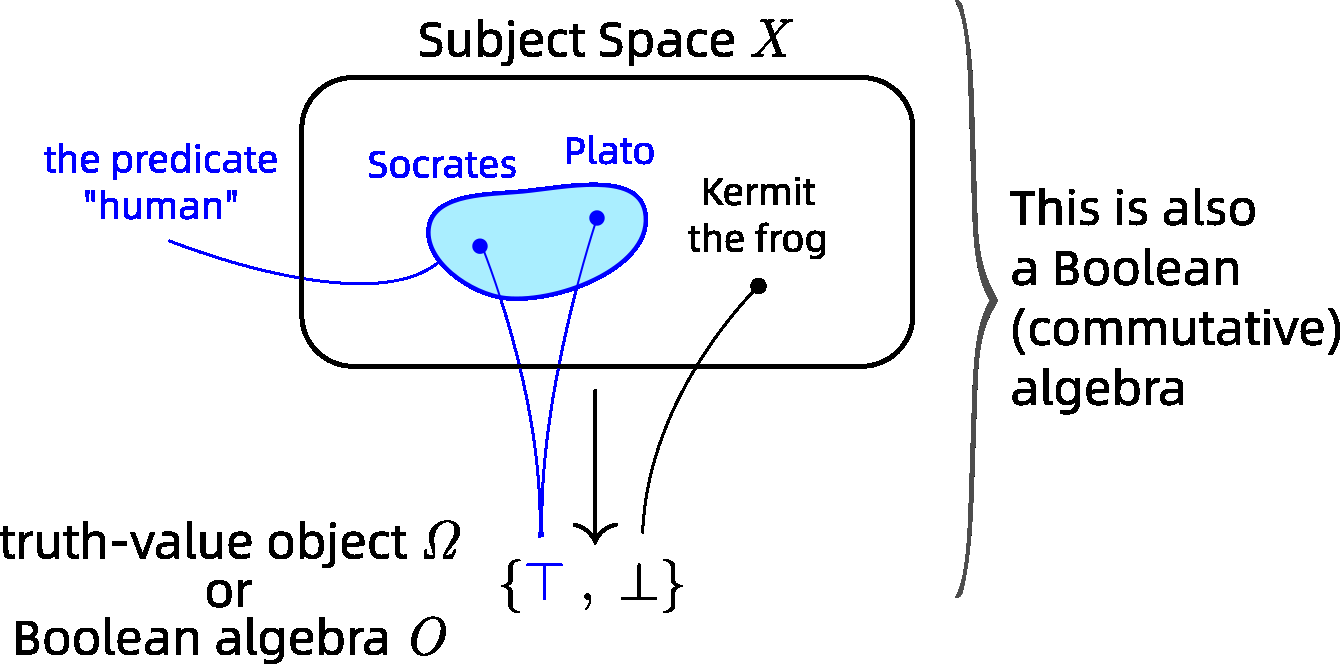
\includegraphics[scale=0.6]{Halmos-nutshell.png}}}
\end{equation}
I coined the term ``Subject Space'' to refer to the space of \textbf{subjects} referred to by predicates.  For example the predicate $\logic{mortal}(\_)$ applies to subjects such as $\logic{Socrates}$ and $\logic{Plato}$ but does not apply to the subject $\logic{Zeus}$.

We all know that propositional logic is isomorphic to the Boolean algebra of sets (Stone's duality theorem).  This is the basis of treating logic as algebra.  But the most sticky point of algebraizing a logic is the treatment of \textbf{predicates}.  Halmos observed that one can form \textbf{propositional functions} from a Subject Space $X$ to a Boolean algebra, and the resulting set of functions would still be a Boolean algebra.  In the above diagram we can see a function mapping subjects to the set $\{ \top, \bot \}$ which is the minimal Boolean algebra $O$, containing only 2 elements, true and false.

The target domain can be a more complex Boolean algebra, as in $X \rightarrow A$.  For example, if Achilles was Zeus's son, he would also be immortal.  So in the proposition space $A$, there would be an implication arrow $\logic{immortal}(\logic{Zeus}) \rightarrow \logic{immortal}(\logic{Achilles})$.  Note that the space $A$ contains points which are just propositions, we cannot access their internal structure.  Anyway, I find that $O = \{ \top, \bot \}$ suffices for our purposes, and we don't need the richer structure of $A$.

More technically, we have the following duality.  Every Boolean algebra $\mathbb{A}$ is isomorphic to the set of all continuous functions from $X$ into $\mathbb{O}$, where $X$ is the dual space of the algebra $\mathbb{A}$, and $\mathbb{O}$ is the Boolean algebra with 2 elements.  If there is a homomorphism $f$ between Boolean algebras $\mathbb{A} \rightarrow \mathbb{B}$ then there is a dual morphism $f^*$ between their dual spaces $Y \rightarrow X$:
\begin{equation}
\begin{tikzcd}[column sep=3cm, row sep=0.6cm]
\mathbb{A} \arrow[r,"f"] \arrow[d,shift left=2,phantom,"\cong"{anchor=south,rotate=90}] & \mathbb{B} \arrow[d,shift left=2,phantom,"\cong"{anchor=south,rotate=90}] \\
\overbracket{X} \arrow[d] & \overbracket{Y} \arrow[d] \arrow[l,"f^*"] \\
\underbracket{\mathbb{O}} & \underbracket{\mathbb{O}} 
\end{tikzcd}
\end{equation}

\section{An ``algebraic geometry'' idea from Yuri Manin and Russians}

Please refer to the next 4 pages excerpted from the book \textit{Geometry I: Basic Ideas and Concepts of Differential Geometry}, by some Russian authors from 1991 \cite{Alekseevskij1991}.  They attributed the idea to Yuri Manin.

My understanding is that \textbf{Boolean algebra} and \textbf{Boolean rings} are essentially synonymous.  Both can be regarded as a form of propositional logic.

\textbf{Stone duality} provides the link between Boolean algebra and the algebra of sets (in a topological space).  But whether this link can be extended to predicate logic is unclear.

\tcbincludegraphics[hbox,colframe=blue,boxrule=1pt,arc=0pt,outer arc=0pt,graphics options={scale=0.5}]{Geometry-I-a.png}

\tcbincludegraphics[hbox,colframe=blue,boxrule=1pt,arc=0pt,outer arc=0pt,graphics options={scale=0.5}]{Geometry-I-b.png}

\tcbincludegraphics[hbox,colframe=blue,boxrule=1pt,arc=0pt,outer arc=0pt,graphics options={scale=0.5}]{Geometry-I-c.png}

\tcbincludegraphics[hbox,colframe=blue,boxrule=1pt,arc=0pt,outer arc=0pt,graphics options={scale=0.5}]{Geometry-I-d.png}


\section{``Term rewriting and all that''}

From the book of that title \cite{Baader1998}.  In Chapter 8, \textit{Gr\"{o}bner bases and Buchberger's Algorithm}, a correspondence is made between Huet's \textbf{higher-order unification} algorithm and Buchberger's algorithm for finding Gr\"{o}bner bases.

An interesting question is whether this correspondence fits into our framework of algebraic logic.  I need more time to determine this...

\begin{equation}
\vcenter{\hbox{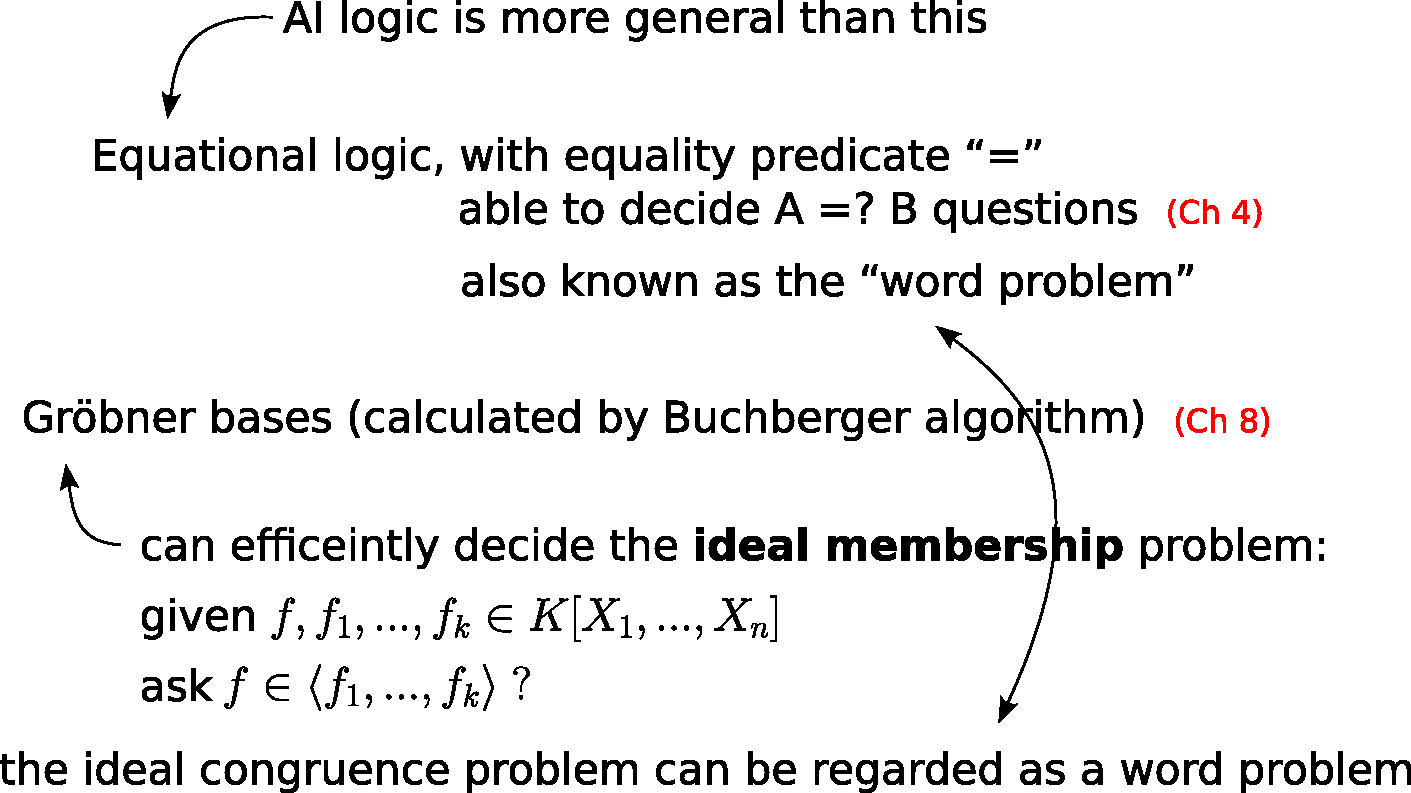
\includegraphics[scale=0.7]{term-rewriting-and-all-that.png}}}
\end{equation}

\begin{itemize}
	\item What is the \textbf{word problem}? \\
	is defined for an equational theory $E$. \\
	is the problem of deciding whether $s = t$
	
	\item why is Gr\"{o}bner basis equivalent to the word problem? \\
	to ask ideal congruence $f =? g$ means $f - g \in? J$ \\
	which is ideal membership problem \\
	a polynomial can be regarded as a rewrite rule \\
	because $f = 0$, we can take the ``largest monomial'' in $f$ as the LHS, and the rest of $f$ as RHS. \\
	In other words:  ideal = set of rules \\
	We ask if a polynomial can be rewritten by the set of rules to another form.  \\
	This is similar to logic deduction.
	
	\item Here an important question is: polynomial reduction seems unable to handle \textbf{logic variables}, it seems only capable of \textbf{simple symbolic rewriting}.
	
	\item logic is equivalent to what form of polynomials? \\
	taking the cue that Huet's higher-order unification = Buchberger algorithm, ...
\end{itemize}

